%%%%%%%%%%%%%%%%%%%%%%%%%%%%%%%%%%%%%%%%%%%%%%%%%%%%%%%%%%%%%%%%%%%%%%%%%%%%%%%%
%%
%% Para utilizar ese modelo sao necessarios os seguintes arquivos:
%%
%% copin.cls
%% copin.sty
%% mestre.sty
%%
%%%%%%%%%%%%%%%%%%%%%%%%%%%%%%%%%%%%%%%%%%%%%%%%%%%%%%%%%%%%%%%%%%%%%%%%%%%%%%%%

\documentclass[a4paper,titlepage]{copin}
\usepackage[portuges,english]{babel}
\usepackage{copin,mestre,epsfig}
\usepackage{times}

%-------------------------- Para usar acentuacaoo em sistemas ISO8859-1 ------------------------------------
% Se estiver usando o Microsoft Windows ou linux com essa codificacao, descomente essa linhas abaixo
% e comente as linhas referentes ao UTF8
\usepackage[latin1]{inputenc} % Usar acentuacao em sistemas ISO8859-1, comentar a linha com  \usepackage[utf8x]{inputenc}
%-----------------------------------------------------------------------------------------------------

%-------------------------- Para usar acentuacao em sistemas UTF8 ------------------------------------
% Para a maior parte das distribuicoes linux, usar a opcao utf8x (lembrar de comentar as linha referente a ISO8859-1 acima)
\usepackage{ucs}
%\usepackage[utf8x]{inputenc}
%\usepackage[utf8]{inputenc}
\usepackage[T1]{fontenc}
%-----------------------------------------------------------------------------------------------------


\usepackage{fancyheadings}
\usepackage{graphicx}
\usepackage{longtable} %tabelas longas, para tabelas que ultrapassam uma pagina
%\input{psfig.sty}


% ----------------- Para inserir codigo fonte de linguagens de programacao no documento -------------
\usepackage{listings}
\lstset{numbers=left,
stepnumber=1,
firstnumber=1,
%numberstyle=\tiny,
extendedchars=true,
breaklines=true,
frame=tb,
basicstyle=\footnotesize,
stringstyle=\ttfamily,
showstringspaces=false
}
\renewcommand{\lstlistingname}{C\'odigo Fonte}
\renewcommand{\lstlistlistingname}{Lista de C\'odigos Fonte}
% ---------------------------------------------------------------------------------------------------

\selectlanguage{portuges}
\sloppy



\begin{document}



%%%%%%%%%%%%%%%%%%%%%%%%%%%%%%%%%%%%%%%%%%%%%%%%%%%%%%%%%%%%%%%%%%%%%%%%%%%%%%%%
\Titulo{T�tulo de sua Disserta��o}
\Autor{Nome do Aluno}
\Data{01/06/2007}
\Area{Ci�ncia da Computa��o}
\Pesquisa{Linha de Pesquisa}
\Orientadores{Nome do Orientador  \\
	 (Orientador)}

\newpage
\cleardoublepage

\PaginadeRosto

\newpage
\cleardoublepage

%%%%%%%%%%%%%%%%%%%%%%%%%%%%%%%%%%%%%%%%%%%%%%%%%%%%%%%%%%%%%%%%%%%%%%%%%%%%%%%%
\begin{resumo} 
Sites \qa são aqueles acessados por usuários com o intuito de: encontrar uma resposta para alguma pergunta ou ajudar alguém a conseguir isto. Tais sites são muito utilizados, por exemplo, por programadores que desejam esclarecer dúvidas gerais sobre programação, como é o caso do site \textit{Stack Overflow em Português}. Muitos pesquisadores têm concentrado esforços visando descobrir maneiras de atrair mais conteúdo para sites deste tipo e, também, entender comportamentos e motivações dos respectivos usuários. Investigou-se, neste trabalho, a utilização da prática do compartilhamento de perguntas oriundas de sites \qa em redes sociais como estratégia para fomentar a contribuição em tais sites. Nosso intuito era: entender como os usuários se comportam diante de tal funcionalidade, investigar como promover tal prática e, por fim, tentar encontrar indícios acerca da utilidade desta prática como meio de fomentar a contribuição em sites \qanospace. Foram feitas duas investigações qualitativas nas quais usuários de sites \qa e de redes sociais foram entrevistados e relataram como se comportam diante do compartilhamento de perguntas. Posteriormente, foi realizado um experimento quantitativo para testar diferentes formas de incentivar o compartilhamento de perguntas oriundas de sites \qa em redes sociais, bem como para investigar mais a fundo o efeito desta prática no conteúdo destes sites. Descobriu-se que os usuários são muito criteriosos na escolha dos conteúdos que eles compartilham nas suas redes sociais por causa dos custos sociais envolvidos. Por este motivo concluímos que é preciso repensar a forma com a qual se tenta promover o compartilhamento de perguntas de tais sites em redes sociais. Além disto, também foi possível perceber que tal compartilhamento pode não ser uma boa escolha para quem pretende fomentar a contribuição nestes sites em questão.
\end{resumo}

\newpage
\cleardoublepage

%%%%%%%%%%%%%%%%%%%%%%%%%%%%%%%%%%%%%%%%%%%%%%%%%%%%%%%%%%%%%%%%%%%%%%%%%%%%%%%%
\begin{summary}
\qa sites are those which are accessed by users who want to find some answer to some question or help someone else to get this. These websites are very used, for instance, by programmers in order to clarify general questions about programming. This behavior could be found in a website called \textit{Stack Overflow em Português}. Many researchers have been focused on finding out ways to attract more content to these websites and, also, on the aspects of behaviors and motivations of its users. In this work our focus was the use of the practice of sharing \qa sites questions in social networks as strategy to increase the content of these websites. Our aim was: to extract some lessons about how is the users' behavior when they face the functionality of to share questions in \qa sites, investigate how to promote this behavior and find out evidences about the advantages for \qa sites related to this practice as way to increase the contribution to this kind of websites. We conducted two qualitative investigations in which users from \qa sites and social networks were interviewed and they related how were they behaviors when they faced the sharing of questions. Then, we made a quantitative experiment in order to test different ways of promoting the sharing of \qa sites questions in social networks, as well as to investigate more deeply the effect of this practice in these websites contents. We found that the users are very discerning when they decide to share or not content in their social networks because of the related social costs. That's why we believe that it's necessary to change the way to promote the sharing of \qa sites questions in social networks. Besides that, it's also possible to notice that this sharing of questions may not be a good strategy to increase the contribution in these websites.  
\end{summary}

\newpage
\cleardoublepage

%%%%%%%%%%%%%%%%%%%%%%%%%%%%%%%%%%%%%%%%%%%%%%%%%%%%%%%%%%%%%%%%%%%%%%%%%%%%%%%%
\begin{agradecimentos}
Agradeço a Deus, sempre, a saúde e as oportunidades que a mim foram dadas. Agradeço aos meus pais, seu Glauco e dona Terezinha, o apoio incondicional e o zelo com o qual a minha educação básica foi tratada desde quando eu nasci. Agradeço aos demais membros da minha família que também me apoiaram, de alguma forma, durante esta minha empreitada.

Agradeço aos amigos do grupo \textit{OFF Thread} a sincera e carinhosa amizade.

Agradeço ao meu orientador, o professor Nazareno Andrade, os valiosos ensinamentos que levarei comigo durante toda a minha jornada profissional.

Agradeço a todos aqueles que participaram das minhas investigações, tanto por meio das entrevistas concedidas quanto por meio da utilização do site \textit{Dê uma Força para o Stack Overflow em Português!}

Agradeço aos professores e colegas pesquisadores do \textit{LSD}, especialmente: Felipe Vieira, Nigini Abilio, Lesandro Ponciano, Milena Araujo e Aline Morais.

Agradeço ao governo brasileiro que, por meio da Coordenação de Aperfeiçoamento de Pessoal de Nível Superior, financiou a minha pesquisa de mestrado durante o último biênio.
\end{agradecimentos}

\clearpage

%%%%%%%%%%%%%%%%%%%%%%%%%%%%%%%%%%%%%%%%%%%%%%%%%%%%%%%%%%%%%%%%%%%%%%%%%%%%%%%%
%% Definicao do cabecalho: secao do lado esquerdo e numero da pagina do lado direito
\pagestyle{fancy}
\addtolength{\headwidth}{\marginparsep}\addtolength{\headwidth}{\marginparwidth}\headwidth = \textwidth
\renewcommand{\chaptermark}[1]{\markboth{#1}{}}
\renewcommand{\sectionmark}[1]{\markright{\thesection\ #1}}\lhead[\fancyplain{}{\bfseries\thepage}]%
	     {\fancyplain{}{\emph{\rightmark}}}\rhead[\fancyplain{}{\bfseries\leftmark}]%
             {\fancyplain{}{\bfseries\thepage}}\cfoot{}

%%%%%%%%%%%%%%%%%%%%%%%%%%%%%%%%%%%%%%%%%%%%%%%%%%%%%%%%%%%%%%%%%%%%%%%%%%%%%%%%
\selectlanguage{portuges}

\Sumario
\ListadeSimbolos
\listoffigures
\listoftables
\lstlistoflistings %lista de codigos fonte - Para inserir a listagem de codigos fonte
\newpage
\cleardoublepage

\Introducao


%%%%%%%%%%%%%%%%%%%%%%%%%%%%%%%%%%%%%%%%%%%%%%%%%%%%%%%%%%%%%%%%%%%%%%%%%%%%%%%%
%
% Hifenizacao - Colocar lista de palavras que nao devem ser separadas e que 
% nao estao no dicionario portugues.
% As palavras do dicionario portugues ja sao separadas corretamente pelo lateX
%
\hyphenation{ Hardware Software etc  }


%%%%%%%%%%%%%%%%%%%%%%%%%%%%%%%%%%%%%%%%%%%%%%%%%%%%%%%%%%%%%%%%%%%%%%%%%%%%%%%%
%% A partir daqui coloque seus capitulos. Sugere-se que eles sejam inseridos com o comando \input
%% Da seguinte maneira:
%%
%% \chapter{Introdução}

\section{Seçãoo 1 do Capítulo 1}
\subsection{Subseção}
\subsubsection{Subsubseção}

A Figura \ref{fig:sistemaProposto}. A Tabela \ref{tab:tabelaTeste}. A Equação (\ref{eq1}). O trabalho de fulano~\cite{ref1}. O Código Fonte \ref{cod1}.

\begin{figure}[htbp]	
\begin{center}
		\fbox{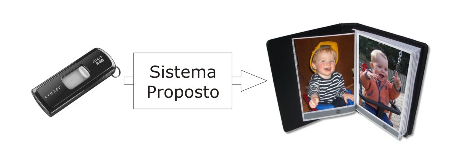
\includegraphics[scale=1]{sistemaProposto.eps}}
	\end{center}
	\caption{Sistema proposto}
	\label{fig:sistemaProposto}
\end{figure}

\begin{table}[htpb]
\begin{center}
\begin{tabular}{|c|c|c|}
\hline
coluna 1 & coluna 2 & coluna 3 \\
\hline
valor 1,1 & valor 1,2 & valor 1,3 \\
valor 2,1 & valor 2,2 & valor 2,3 \\
\hline
\end{tabular}
\end{center}
\caption{Primeira tabela.}
\label{tab:tabelaTeste}
\end{table}

\begin{equation}
E = m \times c^2
\label{eq1}
\end{equation}

\begin{lstlisting}[caption={Loop simples},label=cod1,numbers=none]
for(int x=1; x<10; x++){
  cout << x << "\n";
}
\end{lstlisting}

\section{Seção 2 do Capítulo 1}  
\subsection{Subseção}
\subsubsection{Subsubseção}

 
%% \input{cap2}
\chapter{Introdução}

\section{Seçãoo 1 do Capítulo 1}
\subsection{Subseção}
\subsubsection{Subsubseção}

A Figura \ref{fig:sistemaProposto}. A Tabela \ref{tab:tabelaTeste}. A Equação (\ref{eq1}). O trabalho de fulano~\cite{ref1}. O Código Fonte \ref{cod1}.

\begin{figure}[htbp]	
\begin{center}
		\fbox{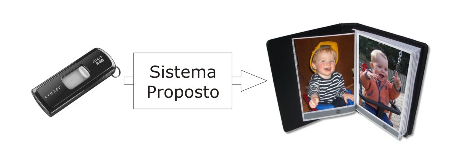
\includegraphics[scale=1]{sistemaProposto.eps}}
	\end{center}
	\caption{Sistema proposto}
	\label{fig:sistemaProposto}
\end{figure}

\begin{table}[htpb]
\begin{center}
\begin{tabular}{|c|c|c|}
\hline
coluna 1 & coluna 2 & coluna 3 \\
\hline
valor 1,1 & valor 1,2 & valor 1,3 \\
valor 2,1 & valor 2,2 & valor 2,3 \\
\hline
\end{tabular}
\end{center}
\caption{Primeira tabela.}
\label{tab:tabelaTeste}
\end{table}

\begin{equation}
E = m \times c^2
\label{eq1}
\end{equation}

\begin{lstlisting}[caption={Loop simples},label=cod1,numbers=none]
for(int x=1; x<10; x++){
  cout << x << "\n";
}
\end{lstlisting}

\section{Seção 2 do Capítulo 1}  
\subsection{Subseção}
\subsubsection{Subsubseção}




%%%%%%%%%%%%%%%%%%%%%%%%%%%%%%%%%%%%%%%%%%%%%%%%%%%%%%%%%%%%%%%%%%%%%%%%%%%%%%%%
%% BIbliografia
%% Coloque suas referencias no arquivo ref.bib e descomente as proximas duas linhas

\bibliographystyle{plain} % estilo de bibliografia   plain,unsrt,alpha,abbrv.
\bibliography{ref} % arquivos com as entradas bib.

%%%%%%%%%%%%%%%%%%%%%%%%%%%%%%%%%%%%%%%%%%%%%%%%%%%%%%%%%%%%%%%%%%%%%%%%%%%%%%%%
%% Apendice
% Caso seja necessario algum apendice, descomente a proxima linha.

\appendix
\chapter{Meu primeiro ap�ndice}

\chapter{Meu segundo ap�ndice}

%%%%%%%%%%%%%%%%%%%%%%%%%%%%%%%%%%%%%%%%%%%%%%%%%%%%%%%%%%%%%%%%%%%%%%%%%%%%%%%%

\end{document}